% Options for packages loaded elsewhere
\PassOptionsToPackage{unicode}{hyperref}
\PassOptionsToPackage{hyphens}{url}
%
\documentclass[
]{article}
\usepackage{amsmath,amssymb}
\usepackage{iftex}
\ifPDFTeX
  \usepackage[T1]{fontenc}
  \usepackage[utf8]{inputenc}
  \usepackage{textcomp} % provide euro and other symbols
\else % if luatex or xetex
  \usepackage{unicode-math} % this also loads fontspec
  \defaultfontfeatures{Scale=MatchLowercase}
  \defaultfontfeatures[\rmfamily]{Ligatures=TeX,Scale=1}
\fi
\usepackage{lmodern}
\ifPDFTeX\else
  % xetex/luatex font selection
\fi
% Use upquote if available, for straight quotes in verbatim environments
\IfFileExists{upquote.sty}{\usepackage{upquote}}{}
\IfFileExists{microtype.sty}{% use microtype if available
  \usepackage[]{microtype}
  \UseMicrotypeSet[protrusion]{basicmath} % disable protrusion for tt fonts
}{}
\makeatletter
\@ifundefined{KOMAClassName}{% if non-KOMA class
  \IfFileExists{parskip.sty}{%
    \usepackage{parskip}
  }{% else
    \setlength{\parindent}{0pt}
    \setlength{\parskip}{6pt plus 2pt minus 1pt}}
}{% if KOMA class
  \KOMAoptions{parskip=half}}
\makeatother
\usepackage{xcolor}
\usepackage[margin=1in]{geometry}
\usepackage{color}
\usepackage{fancyvrb}
\newcommand{\VerbBar}{|}
\newcommand{\VERB}{\Verb[commandchars=\\\{\}]}
\DefineVerbatimEnvironment{Highlighting}{Verbatim}{commandchars=\\\{\}}
% Add ',fontsize=\small' for more characters per line
\usepackage{framed}
\definecolor{shadecolor}{RGB}{248,248,248}
\newenvironment{Shaded}{\begin{snugshade}}{\end{snugshade}}
\newcommand{\AlertTok}[1]{\textcolor[rgb]{0.94,0.16,0.16}{#1}}
\newcommand{\AnnotationTok}[1]{\textcolor[rgb]{0.56,0.35,0.01}{\textbf{\textit{#1}}}}
\newcommand{\AttributeTok}[1]{\textcolor[rgb]{0.13,0.29,0.53}{#1}}
\newcommand{\BaseNTok}[1]{\textcolor[rgb]{0.00,0.00,0.81}{#1}}
\newcommand{\BuiltInTok}[1]{#1}
\newcommand{\CharTok}[1]{\textcolor[rgb]{0.31,0.60,0.02}{#1}}
\newcommand{\CommentTok}[1]{\textcolor[rgb]{0.56,0.35,0.01}{\textit{#1}}}
\newcommand{\CommentVarTok}[1]{\textcolor[rgb]{0.56,0.35,0.01}{\textbf{\textit{#1}}}}
\newcommand{\ConstantTok}[1]{\textcolor[rgb]{0.56,0.35,0.01}{#1}}
\newcommand{\ControlFlowTok}[1]{\textcolor[rgb]{0.13,0.29,0.53}{\textbf{#1}}}
\newcommand{\DataTypeTok}[1]{\textcolor[rgb]{0.13,0.29,0.53}{#1}}
\newcommand{\DecValTok}[1]{\textcolor[rgb]{0.00,0.00,0.81}{#1}}
\newcommand{\DocumentationTok}[1]{\textcolor[rgb]{0.56,0.35,0.01}{\textbf{\textit{#1}}}}
\newcommand{\ErrorTok}[1]{\textcolor[rgb]{0.64,0.00,0.00}{\textbf{#1}}}
\newcommand{\ExtensionTok}[1]{#1}
\newcommand{\FloatTok}[1]{\textcolor[rgb]{0.00,0.00,0.81}{#1}}
\newcommand{\FunctionTok}[1]{\textcolor[rgb]{0.13,0.29,0.53}{\textbf{#1}}}
\newcommand{\ImportTok}[1]{#1}
\newcommand{\InformationTok}[1]{\textcolor[rgb]{0.56,0.35,0.01}{\textbf{\textit{#1}}}}
\newcommand{\KeywordTok}[1]{\textcolor[rgb]{0.13,0.29,0.53}{\textbf{#1}}}
\newcommand{\NormalTok}[1]{#1}
\newcommand{\OperatorTok}[1]{\textcolor[rgb]{0.81,0.36,0.00}{\textbf{#1}}}
\newcommand{\OtherTok}[1]{\textcolor[rgb]{0.56,0.35,0.01}{#1}}
\newcommand{\PreprocessorTok}[1]{\textcolor[rgb]{0.56,0.35,0.01}{\textit{#1}}}
\newcommand{\RegionMarkerTok}[1]{#1}
\newcommand{\SpecialCharTok}[1]{\textcolor[rgb]{0.81,0.36,0.00}{\textbf{#1}}}
\newcommand{\SpecialStringTok}[1]{\textcolor[rgb]{0.31,0.60,0.02}{#1}}
\newcommand{\StringTok}[1]{\textcolor[rgb]{0.31,0.60,0.02}{#1}}
\newcommand{\VariableTok}[1]{\textcolor[rgb]{0.00,0.00,0.00}{#1}}
\newcommand{\VerbatimStringTok}[1]{\textcolor[rgb]{0.31,0.60,0.02}{#1}}
\newcommand{\WarningTok}[1]{\textcolor[rgb]{0.56,0.35,0.01}{\textbf{\textit{#1}}}}
\usepackage{graphicx}
\makeatletter
\def\maxwidth{\ifdim\Gin@nat@width>\linewidth\linewidth\else\Gin@nat@width\fi}
\def\maxheight{\ifdim\Gin@nat@height>\textheight\textheight\else\Gin@nat@height\fi}
\makeatother
% Scale images if necessary, so that they will not overflow the page
% margins by default, and it is still possible to overwrite the defaults
% using explicit options in \includegraphics[width, height, ...]{}
\setkeys{Gin}{width=\maxwidth,height=\maxheight,keepaspectratio}
% Set default figure placement to htbp
\makeatletter
\def\fps@figure{htbp}
\makeatother
\setlength{\emergencystretch}{3em} % prevent overfull lines
\providecommand{\tightlist}{%
  \setlength{\itemsep}{0pt}\setlength{\parskip}{0pt}}
\setcounter{secnumdepth}{-\maxdimen} % remove section numbering
\newlength{\cslhangindent}
\setlength{\cslhangindent}{1.5em}
\newlength{\csllabelwidth}
\setlength{\csllabelwidth}{3em}
\newlength{\cslentryspacingunit} % times entry-spacing
\setlength{\cslentryspacingunit}{\parskip}
\newenvironment{CSLReferences}[2] % #1 hanging-ident, #2 entry spacing
 {% don't indent paragraphs
  \setlength{\parindent}{0pt}
  % turn on hanging indent if param 1 is 1
  \ifodd #1
  \let\oldpar\par
  \def\par{\hangindent=\cslhangindent\oldpar}
  \fi
  % set entry spacing
  \setlength{\parskip}{#2\cslentryspacingunit}
 }%
 {}
\usepackage{calc}
\newcommand{\CSLBlock}[1]{#1\hfill\break}
\newcommand{\CSLLeftMargin}[1]{\parbox[t]{\csllabelwidth}{#1}}
\newcommand{\CSLRightInline}[1]{\parbox[t]{\linewidth - \csllabelwidth}{#1}\break}
\newcommand{\CSLIndent}[1]{\hspace{\cslhangindent}#1}
\ifLuaTeX
  \usepackage{selnolig}  % disable illegal ligatures
\fi
\IfFileExists{bookmark.sty}{\usepackage{bookmark}}{\usepackage{hyperref}}
\IfFileExists{xurl.sty}{\usepackage{xurl}}{} % add URL line breaks if available
\urlstyle{same}
\hypersetup{
  pdftitle={Real data example},
  pdfauthor={Giovanni Saraceno},
  hidelinks,
  pdfcreator={LaTeX via pandoc}}

\title{Real data example}
\author{Giovanni Saraceno}
\date{}

\begin{document}
\maketitle

{
\setcounter{tocdepth}{2}
\tableofcontents
}
\begin{Shaded}
\begin{Highlighting}[]
\FunctionTok{library}\NormalTok{(tidyverse)}
\end{Highlighting}
\end{Shaded}

\begin{verbatim}
## Warning: il pacchetto 'tidyverse' è stato creato con R versione 4.3.2
\end{verbatim}

\begin{verbatim}
## Warning: il pacchetto 'ggplot2' è stato creato con R versione 4.3.3
\end{verbatim}

\begin{verbatim}
## Warning: il pacchetto 'stringr' è stato creato con R versione 4.3.3
\end{verbatim}

\begin{verbatim}
## Warning: il pacchetto 'lubridate' è stato creato con R versione 4.3.2
\end{verbatim}

\begin{Shaded}
\begin{Highlighting}[]
\FunctionTok{library}\NormalTok{(dplyr)}
\FunctionTok{library}\NormalTok{(ggplot2)}
\end{Highlighting}
\end{Shaded}

The data comes from the study of Woodworth et al. (2017), a replication
study of Seligman (2005)`s work which had suggested that positive
psychology interventions, when delivered via the internet, could
increase participants' happiness and decrease their depression relative
to the changes effected by a placebo control.

Their main finding was contrary to that of the original study by
Seligman (2005). All interventions, including the theoretically-neutral
placebo, led to significant increases in happiness and to significant
reductions in depression. The effects of the positive-psychology
interventions were statistically indistinguishable from those of the
placebo.

We have two data sets:

\begin{itemize}
\tightlist
\item
  The first data set (\texttt{ahi-cesd.csv}) comprises 992 point-in-time
  records of the self-reported happiness and depression of 295
  participants, each assigned to one of four intervention groups, in a
  study of the effect of web-based positive-psychology interventions on
  happiness and depression. Each point-in-time measurement consists of a
  participant's responses to the 24 items of the \textbf{Authentic
  Happiness Inventory (AHI)} and to the 20 items of the \textbf{Center
  for Epidemiological Studies Depression (CES-D)} scale. Measurements
  were attempted at the time of each participant's enrollment in the
  study and on 5 subsequent occasions, the last being approximately 189
  days after enrollment.
\end{itemize}

A \emph{total AHI score} is obtained by summing the scores for the 24
items. A \emph{total CES-D score} is obtained by first reversing the
scores of items 4, 8, 12 and 16, and then summing the scores for the 20
items.

The \texttt{ahi-cesd.csv} contains the following variables:

\begin{itemize}
\tightlist
\item
  \texttt{id}: Participant ID.
\item
  \texttt{occasion}: Measurement occasion: 0 = Pretest (i.e., at
  enrollment), 1 = Posttest (i.e., 7 days after pretest), 2 = 1-week
  follow-up, (i.e., 14 days after pretest, 7 days after posttest), 3 =
  1-month follow-up, (i.e., 38 days after pretest, 31 days after
  posttest), 4 = 3-month follow-up, (i.e., 98 days after pretest, 91
  days after posttest), 5 = 6-month follow-up, (i.e., 189 days after
  pretest, 182 days after posttest).
\item
  \texttt{elapsed.days}: Time since enrollment measured in fractional
  days.
\item
  \texttt{intervention}: 3 positive psychology interventions (PPIs),
  plus 1 control condition: 1 = Using signature strengths, 2 = Three
  good things, 3 = Gratitude visit, 4 = Recording early memories
  (control condition).
\item
  \texttt{ahi01}-\texttt{ahi24}: Responses on 24 AHI items.
\item
  \texttt{cesd01}-\texttt{cesd20}: Responses on 20 CES-D items.
\item
  \texttt{ahiTotal}: Total AHI score.
\item
  \texttt{cesdTotal}: Total CES-D score.
\end{itemize}

\begin{Shaded}
\begin{Highlighting}[]
\NormalTok{dat }\OtherTok{\textless{}{-}} \FunctionTok{read.csv}\NormalTok{(}\StringTok{"ahi{-}cesd.csv"}\NormalTok{)}
\FunctionTok{str}\NormalTok{(dat)}
\end{Highlighting}
\end{Shaded}

\begin{verbatim}
## 'data.frame':    992 obs. of  50 variables:
##  $ id          : int  1 1 2 2 2 2 2 2 3 3 ...
##  $ occasion    : int  0 1 0 1 2 3 4 5 0 2 ...
##  $ elapsed.days: num  0 11.77 0 8.02 14.3 ...
##  $ intervention: int  4 4 1 1 1 1 1 1 4 4 ...
##  $ ahi01       : int  2 3 3 3 3 3 3 3 3 3 ...
##  $ ahi02       : int  3 3 4 4 4 4 3 3 3 3 ...
##  $ ahi03       : int  2 4 3 4 4 4 2 3 2 3 ...
##  $ ahi04       : int  3 3 4 4 4 4 3 4 4 4 ...
##  $ ahi05       : int  3 3 2 3 3 4 3 2 2 4 ...
##  $ ahi06       : int  2 4 3 3 3 4 3 3 3 4 ...
##  $ ahi07       : int  3 4 4 4 4 4 3 3 4 4 ...
##  $ ahi08       : int  3 3 3 4 3 3 3 4 3 3 ...
##  $ ahi09       : int  3 3 3 4 4 4 4 3 4 4 ...
##  $ ahi10       : int  2 2 3 3 4 4 4 3 3 3 ...
##  $ ahi11       : int  3 2 2 3 3 4 4 3 2 3 ...
##  $ ahi12       : int  3 3 3 4 4 4 4 3 4 4 ...
##  $ ahi13       : int  4 4 4 4 4 4 4 4 4 4 ...
##  $ ahi14       : int  2 3 3 4 4 4 3 3 3 3 ...
##  $ ahi15       : int  3 3 3 3 3 3 3 3 3 3 ...
##  $ ahi16       : int  3 3 3 4 4 4 4 3 4 4 ...
##  $ ahi17       : int  2 2 3 4 4 4 3 4 3 4 ...
##  $ ahi18       : int  2 3 3 4 4 4 4 4 3 3 ...
##  $ ahi19       : int  3 3 3 4 4 4 4 2 4 4 ...
##  $ ahi20       : int  3 3 3 4 3 4 4 4 3 4 ...
##  $ ahi21       : int  2 3 2 4 4 4 3 4 3 4 ...
##  $ ahi22       : int  2 3 2 3 4 4 3 3 3 4 ...
##  $ ahi23       : int  3 4 4 4 4 4 3 3 3 3 ...
##  $ ahi24       : int  2 2 3 4 4 4 3 3 4 3 ...
##  $ cesd01      : int  2 2 1 3 1 1 2 2 1 1 ...
##  $ cesd02      : int  1 1 1 2 1 1 3 1 1 1 ...
##  $ cesd03      : int  1 1 1 1 1 1 2 2 1 1 ...
##  $ cesd04      : int  4 4 1 3 1 1 1 4 4 4 ...
##  $ cesd05      : int  1 1 1 1 1 1 1 2 2 3 ...
##  $ cesd06      : int  2 1 1 1 1 1 2 1 1 1 ...
##  $ cesd07      : int  1 2 1 2 1 1 2 1 1 1 ...
##  $ cesd08      : int  3 4 1 1 1 4 4 2 4 4 ...
##  $ cesd09      : int  1 1 1 1 1 1 1 1 1 1 ...
##  $ cesd10      : int  1 2 1 1 1 1 1 1 1 1 ...
##  $ cesd11      : int  3 2 2 1 3 2 2 2 2 2 ...
##  $ cesd12      : int  2 4 4 3 4 1 3 4 4 4 ...
##  $ cesd13      : int  2 1 1 1 3 1 3 3 1 2 ...
##  $ cesd14      : int  3 2 1 1 1 1 1 3 2 2 ...
##  $ cesd15      : int  1 1 1 1 1 1 1 1 1 1 ...
##  $ cesd16      : int  2 3 4 3 1 3 3 4 4 4 ...
##  $ cesd17      : int  1 1 1 1 1 1 1 2 1 1 ...
##  $ cesd18      : int  1 1 1 1 1 1 2 2 1 1 ...
##  $ cesd19      : int  2 1 1 1 1 1 1 1 1 1 ...
##  $ cesd20      : int  2 1 1 1 1 1 1 1 1 1 ...
##  $ ahiTotal    : int  63 73 73 89 89 93 80 77 77 85 ...
##  $ cesdTotal   : int  14 6 7 10 13 8 15 12 3 5 ...
\end{verbatim}

The second dataset (\texttt{participant-info.csv}) contains demographic
information about the each of the 295 participants. The data are
suitable for various time-series analyses and between-group comparisons.
It contains the following variables:

\begin{itemize}
\tightlist
\item
  \texttt{id}: Participant's ID.
\item
  \texttt{intervention}: 3 positive psychology interventions (PPIs),
  plus 1 control condition: 1 = Using signature strengths, 2 = Three
  good things, 3 = Gratitude visit, 4 = Recording early memories
  (control condition).
\item
  \texttt{sex}: 1 for female, 2 for female
\item
  \texttt{age}: Participant's age (in years).
\item
  \texttt{educ}: Level of education: 1 = Less than Year 12, 2 = Year 12,
  3 = Vocational training, 4 = Bachelor's degree, 5 = Postgraduate
  degree.
\item
  \texttt{income}: 1 = below average, 2 = average, 3 = above average.
\end{itemize}

Let's load our data sets:

\begin{Shaded}
\begin{Highlighting}[]
\NormalTok{dat\_part }\OtherTok{\textless{}{-}} \FunctionTok{read.csv}\NormalTok{(}\StringTok{"participant{-}info.csv"}\NormalTok{)}
\FunctionTok{str}\NormalTok{(dat\_part)}
\end{Highlighting}
\end{Shaded}

\begin{verbatim}
## 'data.frame':    295 obs. of  6 variables:
##  $ id          : int  1 2 3 4 5 6 7 8 9 10 ...
##  $ intervention: int  4 1 4 3 2 1 3 2 1 2 ...
##  $ sex         : int  2 1 1 1 2 1 1 1 1 1 ...
##  $ age         : int  35 59 51 50 58 31 44 57 36 45 ...
##  $ educ        : int  5 1 4 5 5 5 5 4 4 4 ...
##  $ income      : int  3 1 3 2 2 1 2 2 3 3 ...
\end{verbatim}

First of all, we must join the two data sets together. We can use the
\texttt{tidytable} package (which we already load through the
\texttt{tidyverse} package). The following options are available to join
two data sets:

\begin{itemize}
\tightlist
\item
  Considering one data set we add the other one to the left (i.e., we
  consider the observations in the first data set): \texttt{left\_join}
\item
  Considering one data set we add the other one to the right (i.e., we
  consider the observations in the second data set):
  \texttt{right\_join}
\item
  Considering both data sets we take the intersection (i.e.,
  observations that are in both data sets in the same time):
  \texttt{inner\_join}
\item
  Considering both data sets we take the union (i.e., observations from
  all data sets): \texttt{full\_join}
\end{itemize}

\begin{Shaded}
\begin{Highlighting}[]
\NormalTok{dat\_full }\OtherTok{\textless{}{-}}\NormalTok{ tidytable}\SpecialCharTok{::}\FunctionTok{inner\_join}\NormalTok{(dat, dat\_part, }\AttributeTok{by =} \FunctionTok{c}\NormalTok{(}\StringTok{"id"}\NormalTok{, }\StringTok{"intervention"}\NormalTok{))}
\end{Highlighting}
\end{Shaded}

After joining two data sets, it is a good practice to check the
dimensions of your new data set

\begin{Shaded}
\begin{Highlighting}[]
\FunctionTok{dim}\NormalTok{(dat)}
\end{Highlighting}
\end{Shaded}

\begin{verbatim}
## [1] 992  50
\end{verbatim}

\begin{Shaded}
\begin{Highlighting}[]
\FunctionTok{dim}\NormalTok{(dat\_part)}
\end{Highlighting}
\end{Shaded}

\begin{verbatim}
## [1] 295   6
\end{verbatim}

\begin{Shaded}
\begin{Highlighting}[]
\FunctionTok{dim}\NormalTok{(dat\_full)}
\end{Highlighting}
\end{Shaded}

\begin{verbatim}
## [1] 992  54
\end{verbatim}

Now, let's see the structure of the data set:

\begin{Shaded}
\begin{Highlighting}[]
\FunctionTok{str}\NormalTok{(dat\_full)}
\end{Highlighting}
\end{Shaded}

\begin{verbatim}
## Classes 'tidytable', 'tbl', 'data.table' and 'data.frame':   992 obs. of  54 variables:
##  $ id          : int  1 1 2 2 2 2 2 2 3 3 ...
##  $ occasion    : int  0 1 0 1 2 3 4 5 0 2 ...
##  $ elapsed.days: num  0 11.77 0 8.02 14.3 ...
##  $ intervention: int  4 4 1 1 1 1 1 1 4 4 ...
##  $ ahi01       : int  2 3 3 3 3 3 3 3 3 3 ...
##  $ ahi02       : int  3 3 4 4 4 4 3 3 3 3 ...
##  $ ahi03       : int  2 4 3 4 4 4 2 3 2 3 ...
##  $ ahi04       : int  3 3 4 4 4 4 3 4 4 4 ...
##  $ ahi05       : int  3 3 2 3 3 4 3 2 2 4 ...
##  $ ahi06       : int  2 4 3 3 3 4 3 3 3 4 ...
##  $ ahi07       : int  3 4 4 4 4 4 3 3 4 4 ...
##  $ ahi08       : int  3 3 3 4 3 3 3 4 3 3 ...
##  $ ahi09       : int  3 3 3 4 4 4 4 3 4 4 ...
##  $ ahi10       : int  2 2 3 3 4 4 4 3 3 3 ...
##  $ ahi11       : int  3 2 2 3 3 4 4 3 2 3 ...
##  $ ahi12       : int  3 3 3 4 4 4 4 3 4 4 ...
##  $ ahi13       : int  4 4 4 4 4 4 4 4 4 4 ...
##  $ ahi14       : int  2 3 3 4 4 4 3 3 3 3 ...
##  $ ahi15       : int  3 3 3 3 3 3 3 3 3 3 ...
##  $ ahi16       : int  3 3 3 4 4 4 4 3 4 4 ...
##  $ ahi17       : int  2 2 3 4 4 4 3 4 3 4 ...
##  $ ahi18       : int  2 3 3 4 4 4 4 4 3 3 ...
##  $ ahi19       : int  3 3 3 4 4 4 4 2 4 4 ...
##  $ ahi20       : int  3 3 3 4 3 4 4 4 3 4 ...
##  $ ahi21       : int  2 3 2 4 4 4 3 4 3 4 ...
##  $ ahi22       : int  2 3 2 3 4 4 3 3 3 4 ...
##  $ ahi23       : int  3 4 4 4 4 4 3 3 3 3 ...
##  $ ahi24       : int  2 2 3 4 4 4 3 3 4 3 ...
##  $ cesd01      : int  2 2 1 3 1 1 2 2 1 1 ...
##  $ cesd02      : int  1 1 1 2 1 1 3 1 1 1 ...
##  $ cesd03      : int  1 1 1 1 1 1 2 2 1 1 ...
##  $ cesd04      : int  4 4 1 3 1 1 1 4 4 4 ...
##  $ cesd05      : int  1 1 1 1 1 1 1 2 2 3 ...
##  $ cesd06      : int  2 1 1 1 1 1 2 1 1 1 ...
##  $ cesd07      : int  1 2 1 2 1 1 2 1 1 1 ...
##  $ cesd08      : int  3 4 1 1 1 4 4 2 4 4 ...
##  $ cesd09      : int  1 1 1 1 1 1 1 1 1 1 ...
##  $ cesd10      : int  1 2 1 1 1 1 1 1 1 1 ...
##  $ cesd11      : int  3 2 2 1 3 2 2 2 2 2 ...
##  $ cesd12      : int  2 4 4 3 4 1 3 4 4 4 ...
##  $ cesd13      : int  2 1 1 1 3 1 3 3 1 2 ...
##  $ cesd14      : int  3 2 1 1 1 1 1 3 2 2 ...
##  $ cesd15      : int  1 1 1 1 1 1 1 1 1 1 ...
##  $ cesd16      : int  2 3 4 3 1 3 3 4 4 4 ...
##  $ cesd17      : int  1 1 1 1 1 1 1 2 1 1 ...
##  $ cesd18      : int  1 1 1 1 1 1 2 2 1 1 ...
##  $ cesd19      : int  2 1 1 1 1 1 1 1 1 1 ...
##  $ cesd20      : int  2 1 1 1 1 1 1 1 1 1 ...
##  $ ahiTotal    : int  63 73 73 89 89 93 80 77 77 85 ...
##  $ cesdTotal   : int  14 6 7 10 13 8 15 12 3 5 ...
##  $ sex         : int  2 2 1 1 1 1 1 1 1 1 ...
##  $ age         : int  35 35 59 59 59 59 59 59 51 51 ...
##  $ educ        : int  5 5 1 1 1 1 1 1 4 4 ...
##  $ income      : int  3 3 1 1 1 1 1 1 3 3 ...
##  - attr(*, ".internal.selfref")=<externalptr>
\end{verbatim}

We must make some preprocessing:

\begin{itemize}
\tightlist
\item
  Transform some variable as factor ones: occasion, intervention, sex,
  educ, and income
\item
  Check for NAs and/or outliers
\item
  Remove the all the ahi and cesd variables except for the total
  variables.
\end{itemize}

\begin{Shaded}
\begin{Highlighting}[]
\NormalTok{ahi\_var }\OtherTok{\textless{}{-}} \FunctionTok{colnames}\NormalTok{(dat\_full)[}\FunctionTok{grepl}\NormalTok{(}\StringTok{"ahi"}\NormalTok{, }\FunctionTok{colnames}\NormalTok{(dat\_full))]}
\NormalTok{cesd\_var }\OtherTok{\textless{}{-}} \FunctionTok{colnames}\NormalTok{(dat\_full)[}\FunctionTok{grepl}\NormalTok{(}\StringTok{"cesd"}\NormalTok{, }\FunctionTok{colnames}\NormalTok{(dat\_full))]}

\NormalTok{dat\_full }\OtherTok{\textless{}{-}}\NormalTok{ dat\_full }\SpecialCharTok{\%\textgreater{}\%}
\NormalTok{  dplyr}\SpecialCharTok{::}\FunctionTok{select}\NormalTok{(}\SpecialCharTok{{-}}\FunctionTok{c}\NormalTok{(ahi\_var[}\SpecialCharTok{{-}}\DecValTok{25}\NormalTok{], cesd\_var[}\SpecialCharTok{{-}}\DecValTok{21}\NormalTok{])) }\SpecialCharTok{\%\textgreater{}\%}
  \FunctionTok{mutate}\NormalTok{(}\AttributeTok{occasion =} \FunctionTok{as.factor}\NormalTok{(occasion),}
         \AttributeTok{intervention =} \FunctionTok{as.factor}\NormalTok{(intervention),}
         \AttributeTok{sex =} \FunctionTok{as.factor}\NormalTok{(sex),}
         \AttributeTok{educ =} \FunctionTok{as.factor}\NormalTok{(educ),}
         \AttributeTok{income =} \FunctionTok{as.factor}\NormalTok{(income))}
\FunctionTok{sum}\NormalTok{(}\FunctionTok{is.na}\NormalTok{(dat\_full))}
\end{Highlighting}
\end{Shaded}

\begin{verbatim}
## [1] 0
\end{verbatim}

\begin{Shaded}
\begin{Highlighting}[]
\FunctionTok{summary}\NormalTok{(dat\_full)}
\end{Highlighting}
\end{Shaded}

\begin{verbatim}
##        id         occasion  elapsed.days    intervention    ahiTotal     
##  Min.   :  1.00   0:295    Min.   :  0.00   1:232        Min.   : 32.00  
##  1st Qu.: 74.75   1:147    1st Qu.:  0.00   2:289        1st Qu.: 63.00  
##  Median :147.00   2:157    Median : 14.79   3:210        Median : 74.00  
##  Mean   :147.36   3:139    Mean   : 44.31   4:261        Mean   : 72.79  
##  3rd Qu.:218.25   4:134    3rd Qu.: 90.96                3rd Qu.: 83.00  
##  Max.   :295.00   5:120    Max.   :223.82                Max.   :114.00  
##    cesdTotal     sex          age        educ    income 
##  Min.   : 0.00   1:843   Min.   :18.00   1: 47   1:246  
##  1st Qu.: 4.00   2:149   1st Qu.:35.00   2: 83   2:447  
##  Median :10.00           Median :46.00   3:131   3:299  
##  Mean   :13.14           Mean   :45.04   4:325          
##  3rd Qu.:19.00           3rd Qu.:54.00   5:406          
##  Max.   :55.00           Max.   :83.00
\end{verbatim}

There are no missing values.

Now, we can create some exploratory plots. Let's see the distribution of
the total AHI score divided by type of intervention:

\begin{Shaded}
\begin{Highlighting}[]
\FunctionTok{ggplot}\NormalTok{(dat\_full) }\SpecialCharTok{+}
  \FunctionTok{geom\_boxplot}\NormalTok{(}\FunctionTok{aes}\NormalTok{(}\AttributeTok{y =}\NormalTok{ ahiTotal, }\AttributeTok{fill =}\NormalTok{ intervention))}
\end{Highlighting}
\end{Shaded}

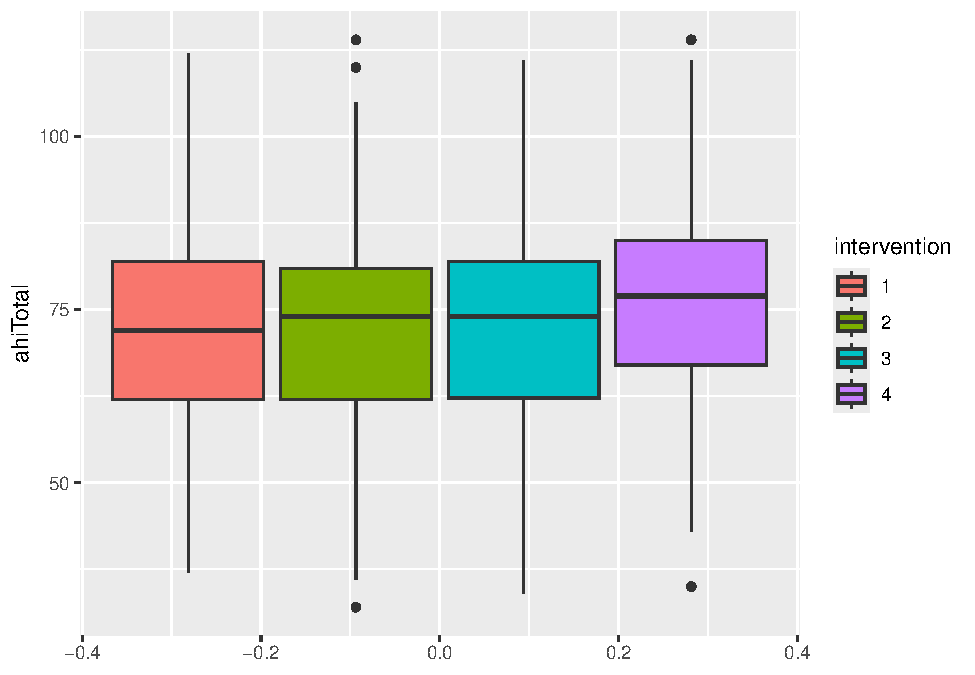
\includegraphics{RealData_example_files/figure-latex/unnamed-chunk-8-1.pdf}

However, we want to see if the total AHI score increases after the
intervention. For simplicity, let's consider the first and second
occasions (i.e., occasion equals 0 and 1):

\begin{Shaded}
\begin{Highlighting}[]
\NormalTok{dat\_full }\SpecialCharTok{\%\textgreater{}\%}
  \FunctionTok{filter}\NormalTok{(occasion }\SpecialCharTok{\%in\%} \FunctionTok{c}\NormalTok{(}\DecValTok{0}\NormalTok{,}\DecValTok{1}\NormalTok{)) }\SpecialCharTok{\%\textgreater{}\%}
  \FunctionTok{ggplot}\NormalTok{() }\SpecialCharTok{+}
  \FunctionTok{geom\_boxplot}\NormalTok{(}\FunctionTok{aes}\NormalTok{(}\AttributeTok{y =}\NormalTok{ ahiTotal, }\AttributeTok{x =}\NormalTok{ intervention}\SpecialCharTok{:}\NormalTok{occasion, }\AttributeTok{fill =}\NormalTok{ occasion))}
\end{Highlighting}
\end{Shaded}

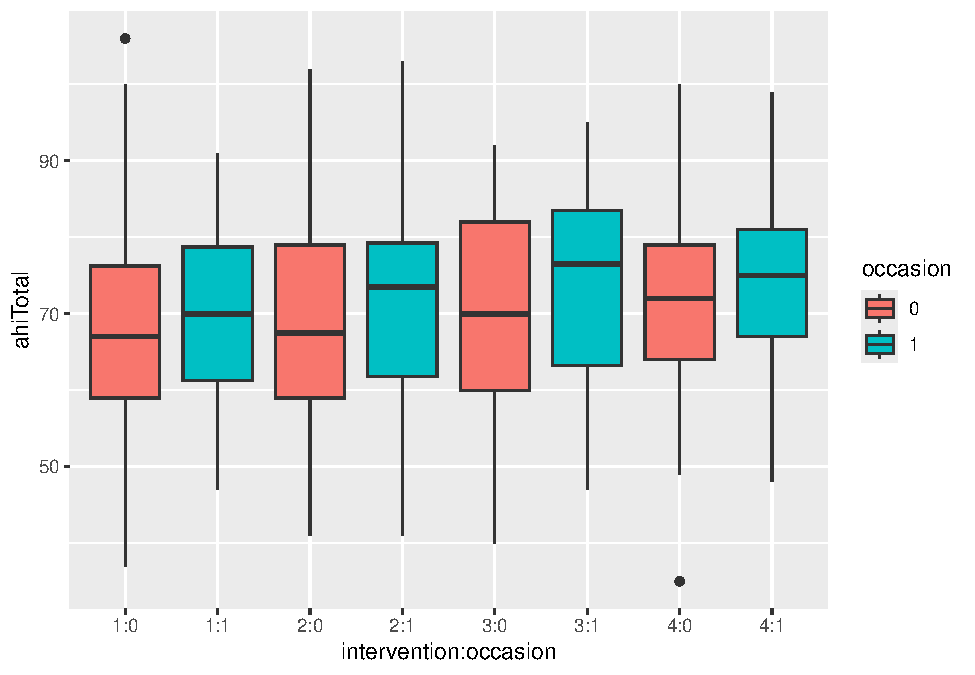
\includegraphics{RealData_example_files/figure-latex/unnamed-chunk-9-1.pdf}

\begin{Shaded}
\begin{Highlighting}[]
  \CommentTok{\#geom\_boxplot(aes(y = ahiTotal, x = intervention:occasion, fill = occasion))}
\end{Highlighting}
\end{Shaded}

We can note an increment of the total AHI score for all the type of
intervetion.

Let's analyze the total CESD one:

\begin{Shaded}
\begin{Highlighting}[]
\NormalTok{dat\_full }\SpecialCharTok{\%\textgreater{}\%}
  \FunctionTok{filter}\NormalTok{(occasion }\SpecialCharTok{\%in\%} \FunctionTok{c}\NormalTok{(}\DecValTok{0}\NormalTok{,}\DecValTok{1}\NormalTok{)) }\SpecialCharTok{\%\textgreater{}\%}
  \FunctionTok{ggplot}\NormalTok{() }\SpecialCharTok{+}
  \FunctionTok{geom\_boxplot}\NormalTok{(}\FunctionTok{aes}\NormalTok{(}\AttributeTok{y =}\NormalTok{ cesdTotal, }\AttributeTok{x =}\NormalTok{ intervention, }\AttributeTok{fill =}\NormalTok{ occasion))}
\end{Highlighting}
\end{Shaded}

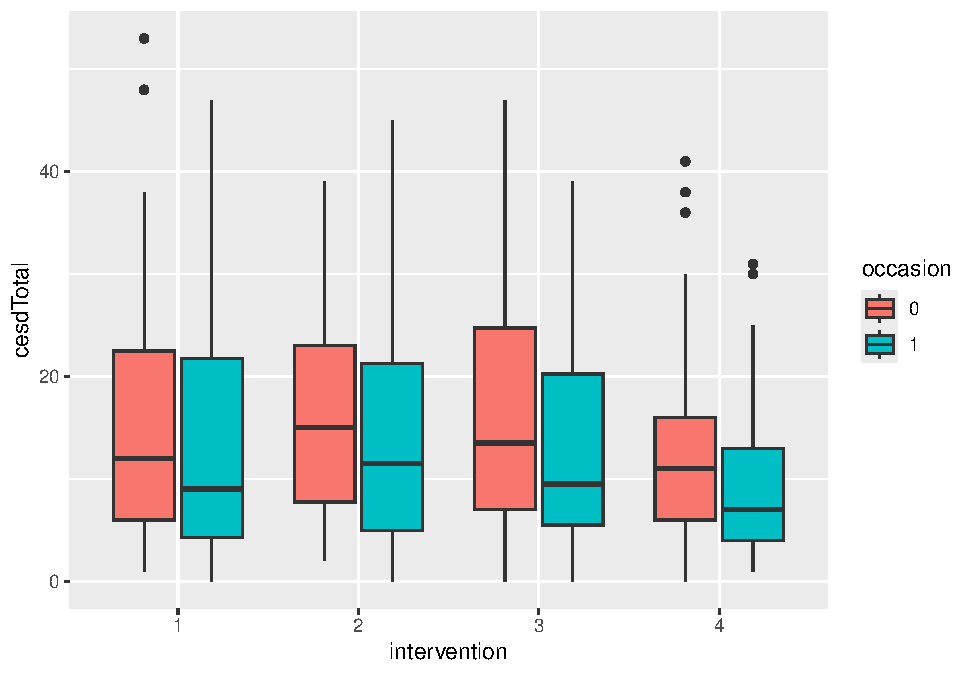
\includegraphics{RealData_example_files/figure-latex/unnamed-chunk-10-1.pdf}

Here, we can see a reduction of the total CESD score for all type of
psychological intervention.

Let's now explore the relationship between the total AHI score and total
CESD score

\begin{Shaded}
\begin{Highlighting}[]
\FunctionTok{ggplot}\NormalTok{(dat\_full) }\SpecialCharTok{+}
  \FunctionTok{geom\_point}\NormalTok{(}\FunctionTok{aes}\NormalTok{(}\AttributeTok{x =}\NormalTok{ ahiTotal, }\AttributeTok{y =}\NormalTok{ cesdTotal)) }\SpecialCharTok{+}
  \FunctionTok{geom\_smooth}\NormalTok{(}\FunctionTok{aes}\NormalTok{(}\AttributeTok{x =}\NormalTok{ ahiTotal, }\AttributeTok{y =}\NormalTok{ cesdTotal), }\AttributeTok{method =} \StringTok{\textquotesingle{}loess\textquotesingle{}}\NormalTok{)}
\end{Highlighting}
\end{Shaded}

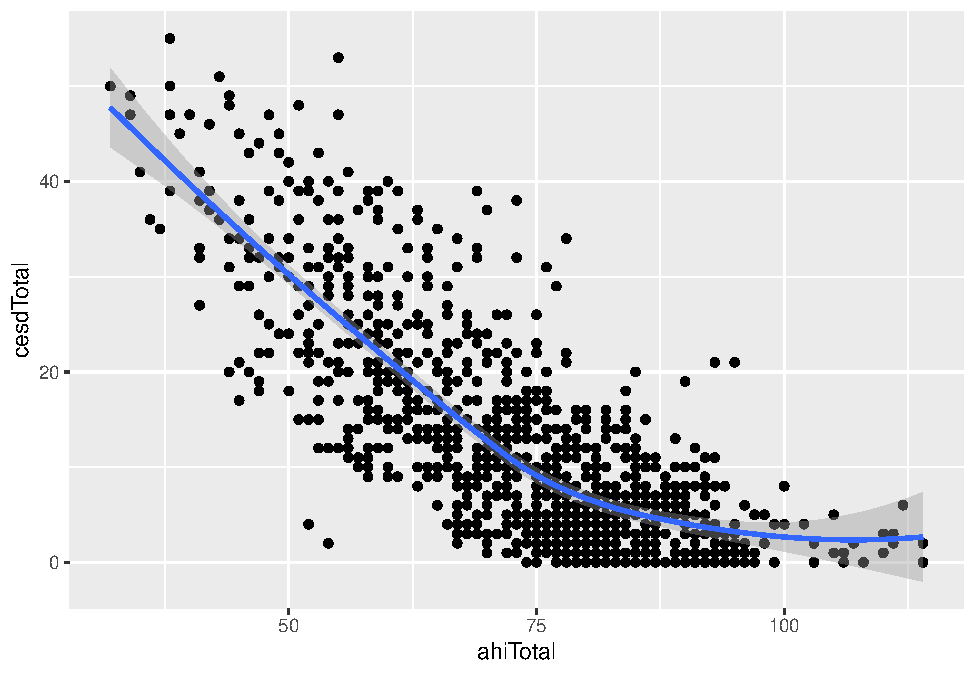
\includegraphics{RealData_example_files/figure-latex/unnamed-chunk-11-1.pdf}

So, high values of AHI correspond to low value of CESD in general.

Another interesting point is to see the total AHI score for each
timepoint and each participants and the mean for each intervention:

\begin{Shaded}
\begin{Highlighting}[]
\NormalTok{dat\_full }\SpecialCharTok{\%\textgreater{}\%}
  \FunctionTok{group\_by}\NormalTok{(intervention, occasion) }\SpecialCharTok{\%\textgreater{}\%}
  \FunctionTok{mutate}\NormalTok{(}\AttributeTok{mean\_ahiTotal =} \FunctionTok{mean}\NormalTok{(ahiTotal)) }\SpecialCharTok{\%\textgreater{}\%}
  \FunctionTok{ggplot}\NormalTok{() }\SpecialCharTok{+} 
  \FunctionTok{geom\_line}\NormalTok{(}\FunctionTok{aes}\NormalTok{(}\AttributeTok{x =}\NormalTok{ occasion, }\AttributeTok{y =}\NormalTok{ ahiTotal, }\AttributeTok{group =}\NormalTok{ id)) }\SpecialCharTok{+}
    \FunctionTok{geom\_line}\NormalTok{(}\FunctionTok{aes}\NormalTok{(}\AttributeTok{x=}\NormalTok{occasion, }
           \AttributeTok{y=}\NormalTok{mean\_ahiTotal, }
           \AttributeTok{group=}\NormalTok{intervention,}
           \AttributeTok{colour=}\NormalTok{intervention), }\AttributeTok{linewidth=}\FloatTok{1.5}\NormalTok{) }
\end{Highlighting}
\end{Shaded}

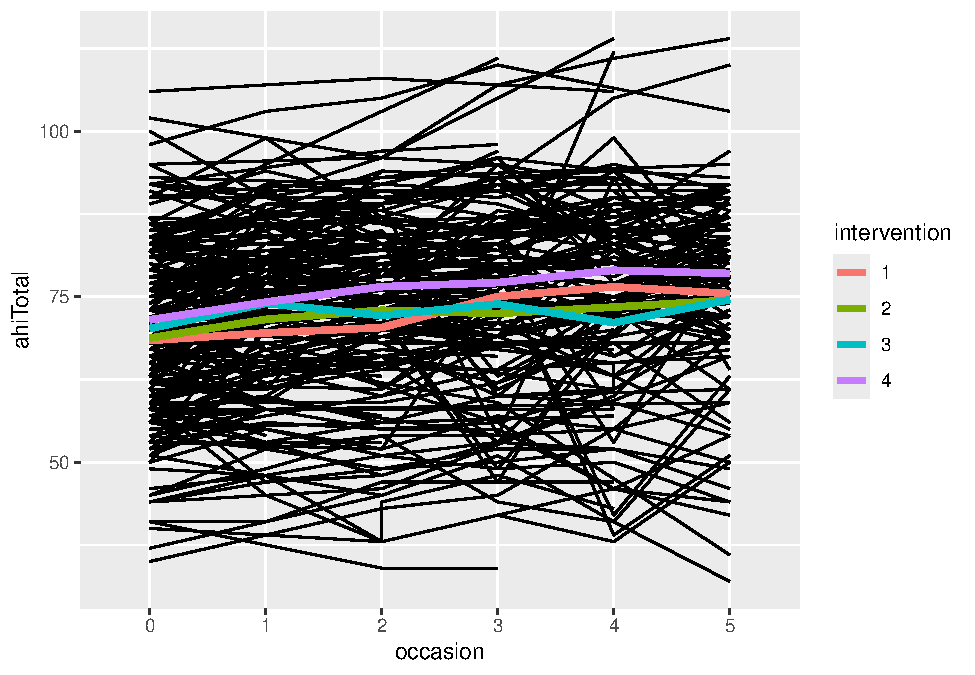
\includegraphics{RealData_example_files/figure-latex/unnamed-chunk-12-1.pdf}

or considering directly the global mean for each occasion and
intervention with corresponding 0.95 confidence intervals:

\begin{Shaded}
\begin{Highlighting}[]
\NormalTok{dat\_full }\SpecialCharTok{\%\textgreater{}\%}
  \FunctionTok{group\_by}\NormalTok{(intervention, occasion) }\SpecialCharTok{\%\textgreater{}\%}
  \FunctionTok{mutate}\NormalTok{(}\AttributeTok{mean\_ahiTotal =} \FunctionTok{mean}\NormalTok{(ahiTotal),}
         \AttributeTok{sd\_ahiTotal=}\FunctionTok{sd}\NormalTok{(ahiTotal),}
         \AttributeTok{n\_ahiTotal=}\FunctionTok{length}\NormalTok{(ahiTotal),}
         \AttributeTok{upper=}\NormalTok{mean\_ahiTotal}\SpecialCharTok{+}\DecValTok{2}\SpecialCharTok{*}\NormalTok{sd\_ahiTotal}\SpecialCharTok{/}\FunctionTok{sqrt}\NormalTok{(n\_ahiTotal),}
         \AttributeTok{lower=}\NormalTok{mean\_ahiTotal}\DecValTok{{-}2}\SpecialCharTok{*}\NormalTok{sd\_ahiTotal}\SpecialCharTok{/}\FunctionTok{sqrt}\NormalTok{(n\_ahiTotal)) }\SpecialCharTok{\%\textgreater{}\%}
  \FunctionTok{ggplot}\NormalTok{() }\SpecialCharTok{+} 
      \FunctionTok{geom\_line}\NormalTok{(}\FunctionTok{aes}\NormalTok{(}\AttributeTok{x=}\NormalTok{occasion, }
             \AttributeTok{y=}\NormalTok{mean\_ahiTotal, }
             \AttributeTok{group=}\NormalTok{intervention,}
             \AttributeTok{colour=}\NormalTok{intervention), }\AttributeTok{size=}\FloatTok{1.5}\NormalTok{) }\SpecialCharTok{+}
    \FunctionTok{geom\_errorbar}\NormalTok{(}\FunctionTok{aes}\NormalTok{(}\AttributeTok{x=}\NormalTok{occasion, }\AttributeTok{ymin=}\NormalTok{upper, }\AttributeTok{ymax=}\NormalTok{lower, }
                      \AttributeTok{color=}\NormalTok{intervention), }
                  \AttributeTok{width=}\FloatTok{0.2}\NormalTok{, }\AttributeTok{linewidth=}\DecValTok{1}\NormalTok{,}\AttributeTok{alpha=}\NormalTok{.}\DecValTok{5}\NormalTok{)}
\end{Highlighting}
\end{Shaded}

\begin{verbatim}
## Warning: Using `size` aesthetic for lines was deprecated in ggplot2 3.4.0.
## i Please use `linewidth` instead.
## This warning is displayed once every 8 hours.
## Call `lifecycle::last_lifecycle_warnings()` to see where this warning was
## generated.
\end{verbatim}

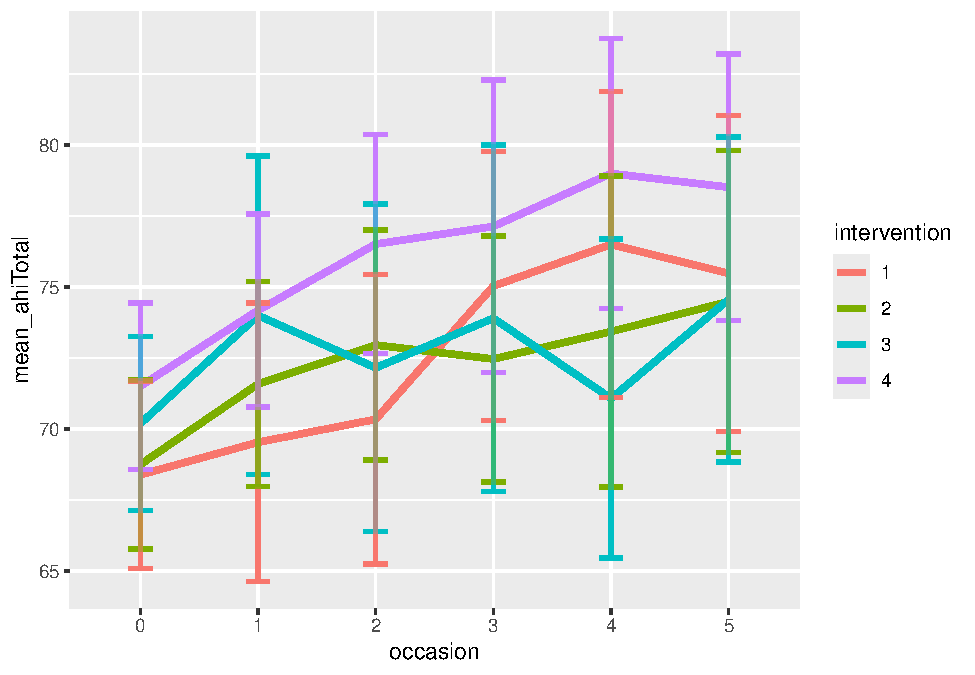
\includegraphics{RealData_example_files/figure-latex/unnamed-chunk-13-1.pdf}

Let's save our preprocessed data set as RData file for the next lesson

\begin{Shaded}
\begin{Highlighting}[]
\FunctionTok{save}\NormalTok{(dat\_full, }\AttributeTok{file =} \StringTok{"dat\_full.RData"}\NormalTok{)}
\end{Highlighting}
\end{Shaded}

\hypertarget{refs}{}
\begin{CSLReferences}{1}{0}
\leavevmode\vadjust pre{\hypertarget{ref-seligman2005}{}}%
Seligman, Steen, M. E. P. 2005. {``Positive Psychology Progress:
Empirical Validation of Interventions.''} \emph{American Psychologist}
60: 410--21.
https://doi.org/\url{https://doi.org/10.1037/0003-066X.60.5.410}.

\leavevmode\vadjust pre{\hypertarget{ref-woodworth2017}{}}%
Woodworth, Rosalind J., Angela O'Brien-Malone, Mark R. Diamond, and
Benjamin Schüz. 2017. {``Web-Based Positive Psychology Interventions: A
Reexamination of Effectiveness.''} \emph{Journal of Clinical Psychology}
73 (3): 218--32.
https://doi.org/\url{https://doi.org/10.1002/jclp.22328}.

\end{CSLReferences}

\end{document}
